\chapter{Real-world Tests}

\section{Metrics}



\subsection{Marginal Likelihood for Modeling}

In our datasets, we use the average log-likelihood as our metric for modeling accuracy.
Given our scene graph model $m$ and hyperparameters $\theta$, the log-likelihood is:
\[
  \mathcal{L} = \sum_{i=1}^N \log p(t_i; x, \theta)
\]


\section{YCB-Video}

\todo


\section{MIT In-House}

\begin{figure}[h]
  \centering
  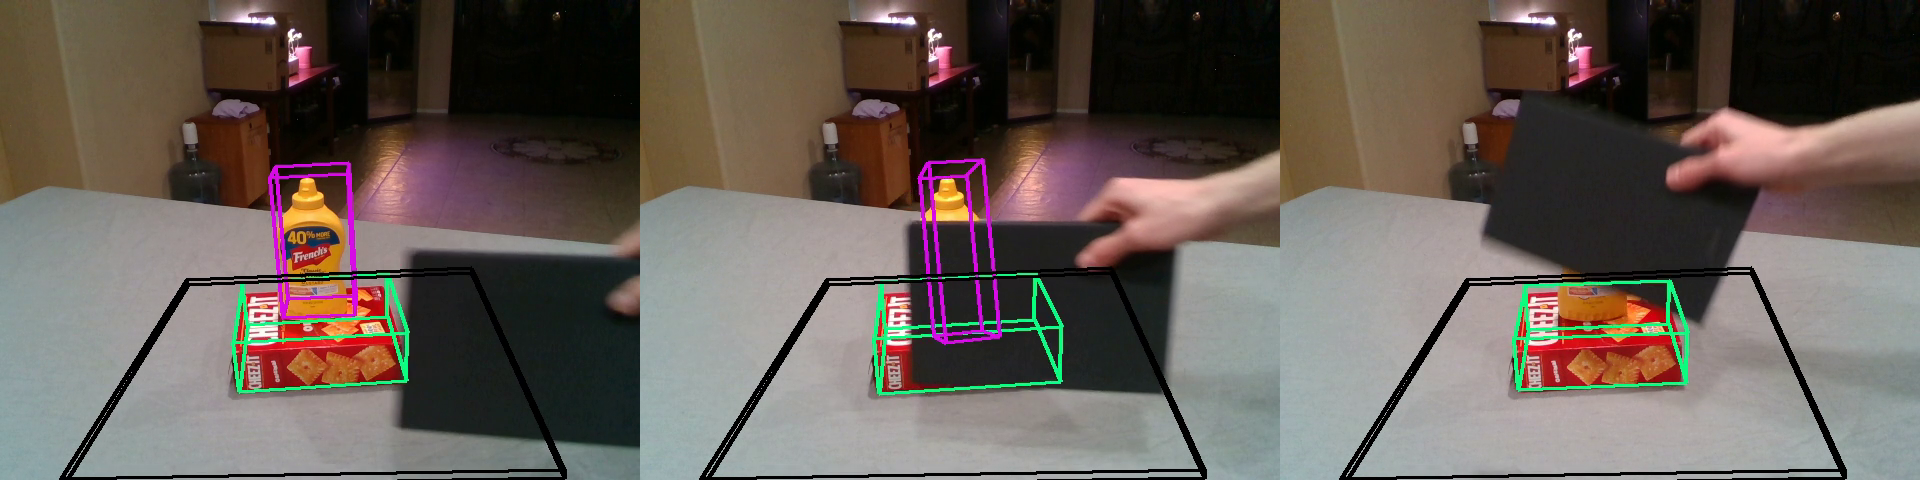
\includegraphics[scale=0.45]{inhouseDataset}
  \caption{
    A selection of frames from sequence \#1, out of 8 captured videos.
    Each sequence contains a different static structure.
    We use a dynamic occluder to generate failure modes in the neural network, in which objects flicker out of existence, or have their poses estimated incorrectly with very large error.
  }
\end{figure}

\subsection{Data Specification}

The YCB-Video data set is a common benchmark for 6 degree of freedom pose estimation, but contains a relatively small number of simple structures.
We'd like to generate additional benchmarks and data for tuning hyperparameters for a richer class of scenes.

\begin{table}
\begin{tabular}{|p{2.5cm}|p{4cm}|p{7.5cm}|}
\hline
\textbf{Name}               & \textbf{Data}          & \textbf{Description} \\
\hline
\textit{Observed poses}              & (String, Vector{Pose}) & nVidia Deep Object Pose Estimator neural detections \\
\hline
Ground truth outlier status & (String, Vector{Bool}) & Per-Frame, per-object flag indicating if an object's neurally generated pose estimate is a noisy outlier \\
\hline
\textit{Ground truth structure}      & Directed Forest        & Observed static structure for the scene  \\
\hline
\textit{Ground truth poses}          & (String, Pose)         & Approximate ground truth static pose, generated as average of inlier DOPE detections \\
\hline
\end{tabular}
\caption{Description of data collected in our real-world experiments with YCB objects.}
\end{table}

We collect a set of experiments with static objects to analyze the model in the static case.
We introduce noise via occluders that block the camera's line of sight to the objects.
The raw video was collected using the Intel RealSense D435 RGB/Depth camera.
Only the RGB information is used for the neural detector, but we collect depth data to enable plane detection, and for future tests on models containing likelihood over depth data.
Observed poses are generated using the publicly provided nVidia DOPE detector GitHub repository.
Ground truth outlier status is manually annotated for each frame in the collected videos.
Note that using the vertices, we can also use the scene graph structure to determine which detections are false positives or negatives.
Ground truth structure is manually annotated once per scene, and the ground truth poses are estimated as the average over all an object's detected \textit{inlier} poses.
While this can potentially obscure systematic bias across all neural detections in the data set, in nonetheless provides a useful relative analysis of the stability of the neural detector in the presence of varying levels of occlusion.
In improving the static version of the model, this could be used as a method to quickly scale the amount of available data for learning model hyperparameters, or even observational model structure.


\subsection{Contact and Noise Hyperparameters}

\begin{figure}[h]
  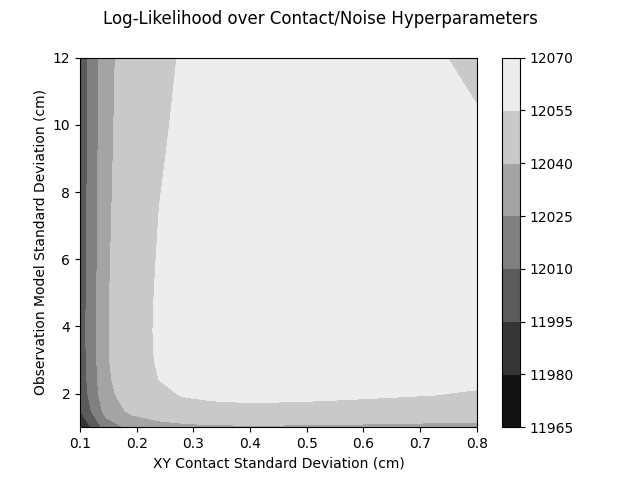
\includegraphics{contactVsNoiseParams}
  \caption{
    Log-likelihood landscape over a grid enumeration of the xy contact model standard deviation, and the observational model standard deviation. The maximum likelihood estimate is located at the star (\todo[Plot the ML estimate for observational model standard deviation versus xy contact standard deviation])
  }
  \label{fig:contactVsNoiseParams}
\end{figure}

\todo

\subsection{Inlier Neural Detection Observational Model}

\begin{figure}[h]
  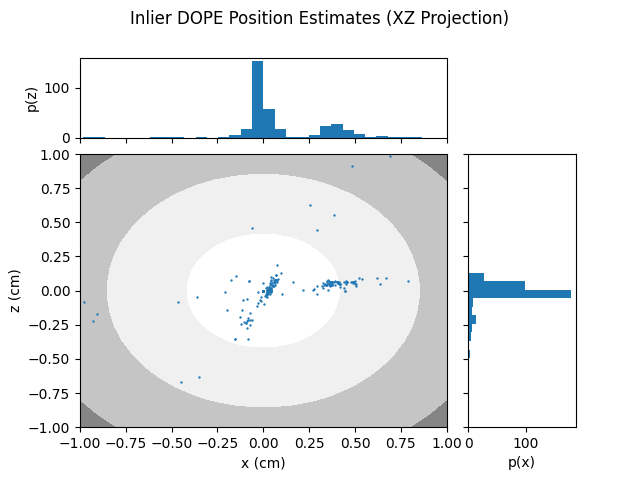
\includegraphics{topdownInlierDetections}
  \caption{
    Scatter plot of the projection of nVidia DOPE's observed pose estimates to the x and z position axes, along with corresponding marginal histograms for each axis respectively.
    The plotted contour is the overlaid noisy observation model for inlier detections (in the projection, a 2D multivariate normal distribution), with the standard deviation hyperparameter set to the maximum-likelihood value as determined in the grid search above.
    Additionally shown are the marginal histograms over the observed poses.
  }
  \label{fig:topdownInlierDetections}
\end{figure}

Figure~\ref{fig:topdownInlierDetections} provides a comparison of a simple observational model in the positional dimensions, fit to maximum likelihood with respect to inlier pose detections. In small deviations from the ground truth, the neural pose estimates exhibit systematic bias in error that could potentially be more accurately represented with a finer-grained observational model.
